\section{Konzept}

\subsection{Web-Framework}
Die Volume Manager Engine soll mit dem Open-Source Web Applikation Framework Ruby on Rails entwickelt werden. Wie der Name dieses Framework beinhaltet basiert Ruby on Rails auf der Programmiersprache Ruby.
Ruby on Rails auch Rails genannt wurde von Dänen David Heinemeier Hannson geschrieben und gilt als Vorbild für weitere Web Applikation Framework wie Grails (Java), CakePhp (PHP), Django (Python) und softies on rails (.Net)  welche die Philosophie von Rails übernommen habe. Die Grund Philosophie von Rails sind die Prinzipien "Don't repeat yourself" kruz DRY und "Convention over configuration".

DRY
Don't Repeat Yourself Philosphie bedeutet das man sich innerhalb der Applikation im Quelltext, in der Konfiguration oder in der Dokumentation nicht wiederholen soll. Mit DRY spart man somit sich Arbeit und gleichzeitig verringert man die Fehleranfälligkeit. Wenn ein Objekt, Funktion oder Konfiguration angepasst werden muss, muss diese nur an einer stelle angepasst werden. Somit muss man sich nicht durch unzählige Daten durchwühlen und es entsteht besserer sauberer und einfach zu warteten Quelltext.


"Convention over configuration"
Eine weit verbreite Eigenschaft von Applikation Framework ist, dass man grosse zum teil komplexe Konfigurationsdateien konfigurieren muss. Rails verhält sich meist fällen so wie man es erwarten würde ohne eine Spezifikation in einer Konfigurationsdatei.  So weiss z.B. der Routing Mechanismus von Rails ohne eine Konfiguration welche Klasse und Methode den Seiten Aufruf abhandle muss. Wo Notwenig können auch Standart verhalten einfach überschrieben werden.

Architektur

\begin{figure}[htb]
\centering
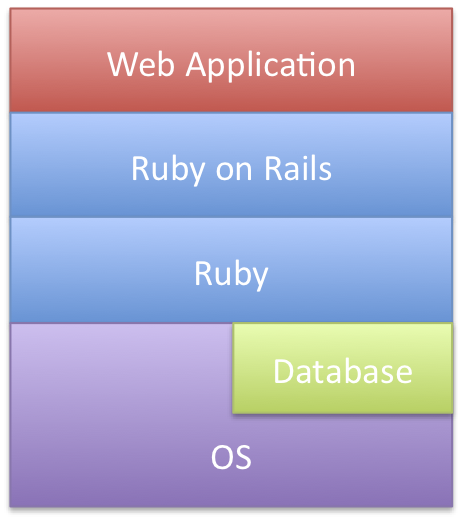
\includegraphics[width=1\textwidth]{RailsApplicationStack.png}
\caption{Rails Architektur: Applikation Stack}
\label{fig:Rails Applikation Stack}
\end{figure}

Alle Rails Applikationen sind nach dem gleichen Grund Architektur aufgebaut, diese ermöglicht es einen neuen Entwickler schneller in der Applikation zurecht finden, wenn er mit Rails vertraut ist. 
Das Design Pattern Model-View-Controll (MVC) teilt die Architektur der Applikation in drei Schichten.

Model
Die Modell Schicht entkoppelt die Daten von der Business Logic zum manipulieren von Daten.

View
Die View Schicht auch Präsentation Schicht stellt das User-Interface der Applikation dar. 

Controler
Die Controller Schicht ist dazu verantwortlich, die Daten von der Benutzereingabe und externer Input zu interpretieren indem die Controller Schicht mit dem beiden Schichten View und Model kommunizieren.






Sortieren und Suchen mit Searchlogic.
Searchlogic macht den gebrauch vonActiveRecord named scopes einfacher und weniger wiederholend. Es hilft den Code einfach uns sauber zu halten (DRY). 

http://github.com/binarylogic/searchlogic

Installation:
\Shell{ sudo gem install searchlogic}

\Shelle{# config/environment.rb
config.gem "searchlogic"}

